%%==========================
%% chapter01.tex for SJTU Master Thesis
%% based on CASthesis
%% modified by wei.jianwen@gmail.com
%% version: 0.3a
%% Encoding: UTF-8
%% last update: Dec 5th, 2010
%%==================================================

%\bibliographystyle{sjtu2} %[此处用于每章都生产参考文献]
\chapter{绪论}
\label{chap:intro}

\section{课题研究背景}
\label{sec:backgroud}

\subsection{大数据}
在现今互联网规模和技术随着时间不断发展的背景下,当今世界的数据量以极快的速度增长。国际数据公司(IDC)\upcite{gantz2010digital}的研究结果表明,2008年全球产生的数据量为0.49ZB,2009年的数据量为0.8ZB,2010年增长为1.2ZB,2011年的数量更是高达1.82ZB\upcite{villars2011big},相当于全球每人产生200GB以上的数据。我们已经进入了一个大数据时代,需要管理的数据资源变得越来越庞大。IBM的一项研究称,整个人类文明所获得的全部数据中,有90\%是在过去的两年产生的,预计到2020年,全世界所产生的数据规模将是今天的44倍。数据如此庞大的特点使得那些分析大数据的工具有很好的生态圈。在开源界,主要有Hadoop HDFS、MapReduce、HBase等等生态圈的形成,另外以Nosql为代表的海量数据管理的技术的应用越来越广泛,比如membase、MongoDB。在商业生态圈里,数据仓库技术越发成熟。

大数据有四个显著的特点,他们分别是量大、繁多、价值密度低、时效性高。在这样的环境下,互联网用户每天会产生海量的数据,传统的基于磁盘文件系统已经无法达到现实意义下的需求,比如可拓展性差和容错性差,取而代之的是分布式文件系统。分布式文件系统是指系统管理的文件资源并不在本地,而是通过计算机网络与本地节点相连。随着分布式文件系统的逐渐壮大,国内很多互联网公司纷纷采用了这样的架构,并且提出了很多很有挑战性的问题。在本文中,对价值密度低这点的一个方面做出相对较好的改善,互联网上有大量重复的数据,导致重复的上传,重复的存储,浪费了巨大的流量和空间。本课题将研究云文件系统存储大数据的同时,如何有效地检测重复数据,将改进现有的做法,提出一种较新的方法来解决这个问题。

\subsection{内存计算}
在现今大数据的时代背景下,内存计算变得越来越普遍,并且也是今后计算的趋势所在。在传统的计算模型下,程序请求数据一般都在磁盘上,导致了需要先从磁盘加载到内存这一步,往往在这是大多数系统的瓶颈所在。在内存计算完以后,还可能需要将计算的结果存会磁盘,比如说一般的数据库操作,那么这一步也将可能是瓶颈的发生点。所以在这样的计算模型下,将无法适应于大数据高时效性的场景。内存计算的做法是,将所有运算结果尽可能保存在内存中从而减少磁盘I/O带来的延迟。而现在越来越多的基于内存计算的计算平台也慢慢出现,比如spark和hadoop。spark是比hadoop晚出现的一个计算框架,在速度上远远超过了hadoop,所以本文主要讨论spark。本文将把本文提出的算法应用到spark平台上,以达到数据处理加速的效果。在未来越来越多的数据场景下,内存计算将越来越占据主导地位。

\section{课题研究内容}
\subsection{课题研究重点}
\label{sec:point1}
各种云文件系统上都存在着大量的重复数据,可能的来源是用户对热门且常见数据的重复上传,也有可能是一些恶意上传者对服务器的攻击,有统计研究表明,有效地检测和删除重复数据,将使得存储资源减少到现在的二十分之一,而且还能很大程度上提高服务器带宽利用率。本课题将着重研究在云文件系统中重复文件的检测和删除技术,结合现有成熟的技术,并深入分析现有算法的优缺点,提出一种基于快速傅里叶变换的相似数据的检测。在传统的技术中,一个文件块的任意一个字节的变动将被视为两个完全不相关的数据,但这个假设在一些情景下是不成立的,传统的算法无法给出一个可伸展可配置的解决方案。在本课题中,将创新性地提出一个系统参数 $\epsilon$ 用于指定用户在特定场景下的近似度,在不同场景设定不同的系统参数将提供用户或管理员很大的灵活性。本文基于内存计算背景下的重复数据删除,研究重点如下:

\begin{enumerate}
\item 不同于传统方法的重复数据检测删除技术

在现有的做法普遍采用了提取特征值的方法,比如说最常见的一种是计算文件的哈希值,经过调研,国内很多厂商都采用这种传统的做法,比如迅雷云盘,百度网盘,又拍云存储等等,在一些场景下,这样的做法高效快速,并能取得很好的效果,其缺点是当文件数量达到一定程度以后,很可能会发生哈希碰撞,比如MD5已被我国山东大学的王晓云教授等人破解,一些恶意的攻击者很有可能利用这一点来攻击服务器,使得服务器上存储着大量的垃圾数据。另一方面,基于特征值的方法无法提供可伸展性,若有任意一点的不同,将被视为重复文件,这在某些场景下是不成立的,一个典型的例子是新闻检测系统,如果一篇针对某一个话题的报道已经上传,那么第二篇相似或重复的报道就应该检测出来。本文将给出基于一个系统参数 $\epsilon$ 的解决方案。

\item 检测相似向量的技术

业界有比较多的解决方案,比如余弦定理。在数学意义上,余弦定理计算的是两个N维向量夹角的余弦值。而在早些时候余弦定理被GOOGLE用来作为新闻分类的重要工具,将新闻的出现的关键字出现的频率提取出来,把它们转化为N维向量,作为这篇新闻的特征值向量,然后计算两篇新闻的特征值向量的余弦值,夹角越小,说明它们越相似。本文将采取相关的算法才判断相似数据。

\item 基于内存计算的计算框架

本课题将计算过程放在spark平台上运行。spark是类Hadoop MapReduce的通用并行框架,Spark基于map reduce算法实现的分布式计算,拥有Hadoop MapReduce所具有的优点;但不同于MapReduce的是Job中间输出和结果可以保存在内存中,从而不再需要读写HDFS,因此Spark能更好地适用于数据挖掘与机器学习等需要迭代的map reduce的算法。spark有如下优点,首先,Spark的中间数据放到内存中,对于迭代运算效率更高。其次,Spark比Hadoop更通用。另外,spark具有更好的容错性和可用性。(这里还能适当扩展http://tech.uc.cn/?p=2116)

\end{enumerate}

\subsection{课题研究难点}
\label{sec:point2}

\begin{enumerate}
\item 快速傅里叶变换(fast fourier transform)的研究和应用

本文的一个难点是是理解把文件块作为离散的点组成的信号,进行傅里叶变换以后是文件的另外一种表达方式,我们利用这种表达方式来对文件块进行处理。

\item 对文件进行预处理以适应FFT

文件块无法直接应用于FFT,需要进行必要的预处理。本文将提出一种简单易懂可行性高的预处理方法。
\end{enumerate}

\section{国内外研究工作}
\label{sec:relatedwork}

在现有的文件去重领域,对数据进行重复数据检测原理大致可以分为五个步骤:

\begin{enumerate}
    \item 数据划分

        将文件文件按照实现约定好的分块策略分成一个个小的文件块。文件块越小,检测强度越高,随之带来的缺点是管理变得复杂。

    \item 特征选择

        对于每一个文件块都找到一个特征值来表示它,对特征值的期望是希望这个值能唯一地表示这个文件块内容,一般选择位数比较多的哈希算法来实现这个目的,比如MD5和SHA1等算法,有的学者因为哈希的碰撞问产生疑虑\cite{henson2003analysis},对于一般使用情况SHA1足以胜任。

    \item 相同检测

        对文件块的特征值和存储的特征值进行比较以确定相同的数据。这一步很容易成为整个重复数据检测过程中的瓶颈所在。

    \item 冗余消除

        通过相同检测,如果发现有相同的文件块,那么就不用保存这个文件块,只需要将指针指向已经保存下来的文件块即可,这样就实现了重复数据的存储和检测。

    \item 数据存储

        将不重复的文件块保存在磁盘上,然后将这块文件块的特征值加到库中,供下一次检测时候使用。
\end{enumeate}

在IBM的一篇Research Report\upcite{denehy2003duplicate}中,举了几个运用这些步骤的算法的例子。
\section{本文主要的工作和创新}
\label{sec:relatedwork}

当前互联网环境下有大量的重复冗余数据,如果用好重复数据的检测和删除技术的话,将大大地提高存储利用率和网络带宽。本文分析了现有做法的一些局限性,并应用文件分块技术,快速傅里叶变换技术,N维向量的相似性检测,spark内存计算等关键技术提出一种基于FFT的相似文件检测技术。最后,本文实现了服务的基本框架,供用户上传文件和重复检测。本文算法的主要流程如\ref{fig:arch}所示。

\begin{figure}[!hbp]
\centering
    \begin{minipage}[b]{1\textwidth}
    \captionstyle{\centering}
    \centering
    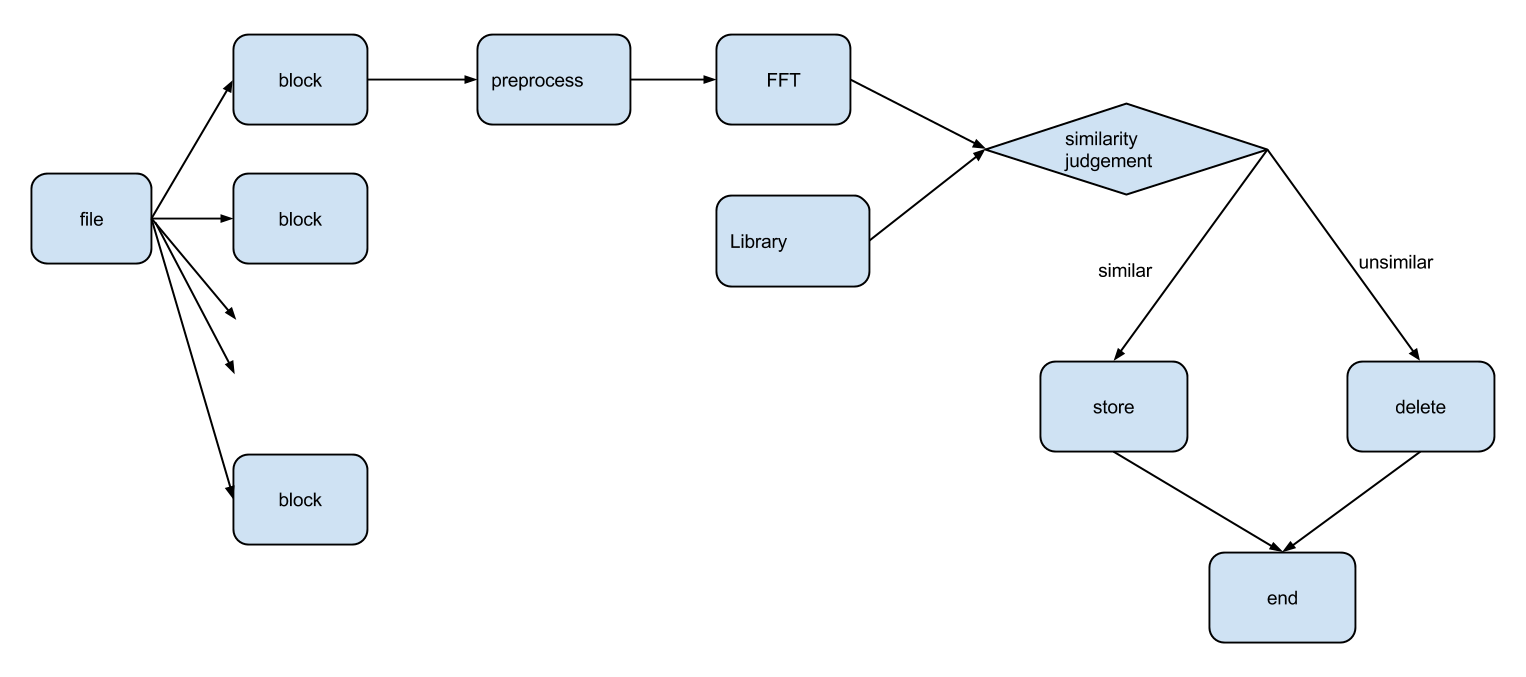
\includegraphics[origin=br,width=16cm]{chap1/archti.png}
    \bicaption[fig:arch]{算法架构}{基于FFT的文件去重算法架构.}{Fig}{Archtecture.}
    \end{minipage}     
\end{figure}

\section{本文的主要结构}
\label{sec:cons}

第一部分为绪论,介绍了课题的的研究背景、课题的研究内容、国内外的研究现状和本文的主要工作和创新。

第二部分为重复数据检测的关键技术,主要讨论了全文件检测技术、简单分块技术、  内容块技术和滑动块技术,最后总结和归纳了这些技术的优缺点以及技术使用场景的局限性。

第三部分介绍了核心技术和内存计算的框架,然后介绍了快速傅里叶变换,以及比较两个N维向量的基础,最后还介绍了基于内存计算的几个框架的比较。

第四部分是基于FFT的相似文件检测算法的提出,我们将先后讨论分块的方法、分块预处理的技术、对文本进行FFT变换的意义和N维向量相似度的比较技术,最后我提出了基于spark的算法设计。

第五部分是系统的实现,并且采用了Client/Server模型作为我们系统服务的最基础的原型。
